\documentclass{article}
\usepackage{graphicx} % For adding images / pdfs
\usepackage[french]{babel} % So that latex generated text follow french language rules
\usepackage[T1]{fontenc} % Font encoding
\usepackage[utf8]{inputenc}
\usepackage[table,xcdraw]{xcolor} % Adds color commands

\usepackage{titlesec} % To modify section title formatting
\usepackage[skip=0.5em, indent=2em]{parskip} % To change paragraph skip
\usepackage{listings} % To add python code (or other languages)
\usepackage{enumitem} % To enumerate over items
\usepackage{caption} % To have modifiable captions under figures
\usepackage{hyperref} % To have clickable references in the text using \ref{}

\usepackage{amsmath} % Adds math expressions
\usepackage{physics} % Adds physics expressions (like derivatives)

\usepackage[per-mode=fraction]{siunitx} % Adds commands for formatting numbers
\usepackage{booktabs} % Adds commands for formatting tables.
\usepackage{makecell} % Adds the \makecell command, useful for to tables (multiple rows of text in a cell)
\usepackage{multicol} % To have 2 columns or more

\usepackage{lipsum} % Lorem ipsum dummy text

%%% PYTHON %%%
% Default fixed font does not support bold face
\DeclareFixedFont{\ttb}{T1}{txtt}{bx}{n}{12} % for bold
\DeclareFixedFont{\ttm}{T1}{txtt}{m}{n}{12}  % for normal

% Custom colors
\usepackage{color}
\definecolor{deepblue}{rgb}{0,0,0.5}
\definecolor{deepred}{rgb}{0.6,0,0}
\definecolor{deepgreen}{rgb}{0,0.5,0}

% Python style for highlighting
\newcommand\pythonstyle{\lstset{
language=Python,
basicstyle=\ttm,
morekeywords={self},              % Add keywords here
keywordstyle=\ttb\color{deepblue},
emph={MyClass,__init__},          % Custom highlighting
emphstyle=\ttb\color{deepred},    % Custom highlighting style
stringstyle=\color{deepgreen},
frame=tb,                         % Any extra options here
showstringspaces=false
}}

% Python environment
\lstnewenvironment{python}[1][]
{
\pythonstyle
\lstset{#1}
}
{}
%%% END PYTHON %%%

%%% Figures %%% -> Replaces the standard "figure" environment so that figures can be added in columns
\newenvironment{Figure}
  {\par\medskip\noindent\minipage{\linewidth}}
  {\endminipage\par\medskip}

%%% Margins %%%
\usepackage[top=1.8cm,bottom=1.8cm,left=1.8cm,right=1.8cm,includehead=true,headheight=0cm,headsep=0cm,footskip=2\normalbaselineskip,showframe=false]{geometry}

%%% Biblatex %%% -> for generating references and citations (significantly increases compile time)
\usepackage[backend=biber,
style=numeric,
sorting=none
]{biblatex}
\addbibresource{refs.bib}

%%% Section numbering %%%
\renewcommand{\thesection}{\Roman{section}.}
\renewcommand{\thesubsection}{\Roman{section} \Alph{subsection}.}
\titleformat{\subsection}
  {\normalfont\normalsize\bfseries\filcenter}{\Alph{subsection}.}{1em}{}
\titleformat{\section}
  {\normalfont\Large\bfseries\filcenter}{\thesection}{1em}{}

%%% Page numbering %%%
\pagenumbering{arabic}

%%% Column width %%%
\setlength{\columnsep}{0.05\textwidth}




\begin{document}

\begin{titlepage}
\begin{center}
    \Large
    Université du Québec à Trois-Rivières

    \vspace{2.5cm}

    \LARGE
    \textbf{Rapport de laboratoire:} \vspace{0.25em}

    \textbf{TITRE}

    \vspace{2.5cm}

    \Large
    Par:\\
    \textit{NOM PRÉNOM} (CODE PERMANENT)

    \vfill

    Travail présenté à:\\
    \vspace{1em}
    \textit{PROFESSEUR}\\
     \vspace{1em}
    Dans le cadre du cours : CODE COURS (ex:PHQ1027)\\
    NOM COURS\\

    \vspace{2.5cm}

    Baccalauréat en physique (7724)\\
    Département de biochimie, chimie, physique et science forensique

    \vspace{2.5cm}


    MOIS ANNÉE

\end{center}
\end{titlepage}



\section*{\hfill Résumé \hfill}
\lipsum[1]


\begin{multicols}{2}
\section{Introduction}

\lipsum[2]


\subsection{Théorie}

\lipsum[3]


\subsection{Autre section si nécessaire}

\begin{align}
    F_f &= {-k}v_0 \nonumber\\
    F_g &= -mg \nonumber
\end{align}

\noindent où $F_f$ est ...

\begin{Figure}
    \centering
    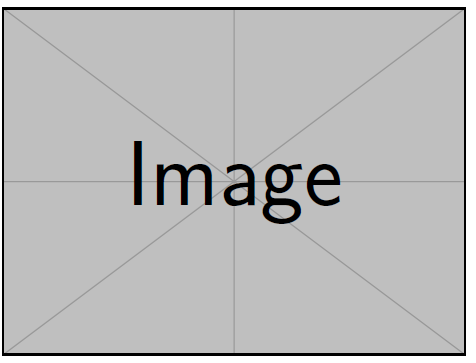
\includegraphics[width=0.4\linewidth]{Figures/dummy.png}
    \captionof{figure}{\textbf{Image}}
    \label{fig: forces pas E}
\end{Figure}


\section{Matériel et méthodologie} \label{sec: méthodo}

\begin{enumerate}[leftmargin=*]
    \item Première étape
    \item Deuxième étape
\end{enumerate}

\noindent \textit{Théorie et manipulations tirées de  \cite{hamelin_physique_nodate}.}

\section{Résultats} \label{sec: résultats}

\lipsum[54]

\begin{Figure}
\centering
\captionof{table}{\textbf{Tableau super cool}}
\label{tab:super cool}
\sisetup{separate-uncertainty=true}
\begin{tabular}{
    c|
    S[table-format=-2.3(1.3)]
    S[table-format=6(5)]
}
\toprule
\toprule
{Série} & {$q$ $(\SI{e-99}{\coulomb})$} & {$\vec E$ $(\SI{e99}{\volt\per\meter})$} \\
\midrule
    1   & 12.7+- 0.4        & 100000+- 30000  \\
    2   & -12.65+- 0.04     & 100000+- 30000 \\
    3   & 12.65+- 0.08      & 100000+- 30000 \\
    4   & 12.653+- 0.002    & 100000+- 30000  \\
\midrule
\midrule
\end{tabular}
\end{Figure}

\section{Discussion} \label{sec:discussion}
\lipsum[4-6]

\section{Conclusion} \label{sec:conclusion}
\lipsum[7]

\end{multicols}

%%%%%%% References  %%%%%%%
\stepcounter{section}
\printbibliography[title={\thesection \quad Références}]
\newpage

%%%%%%% Starting appendix  %%%%%%%
\appendix
\renewcommand{\thesection}{Annexe \Alph{section}.}
\renewcommand{\thesubsection}{\Alph{section} \Roman{subsection}.}
\titleformat{\subsection}
  {\normalfont\normalsize\bfseries}{\thesubsection}{1em}{}
\titleformat{\section}
  {\normalfont\Large\bfseries\filcenter}{\thesection}{1em}{}

\begin{multicols}{2}

\section{Calculs} \label{sec:calculs}

\begin{equation}
    R_{ik} = 8\pi\left( T_{ik} - \tfrac{1}{2}g_{ik}T \right) - \Lambda g_{ik}
\end{equation}

\lipsum[10-12]

\end{multicols}


\section{Tableaux} \label{sec:tableaux}

\begin{table*}[ht]
\centering

\caption{\textbf{Tableau super grand}}
\label{tab:super grand}
\begin{tabular}{cc|ccc}
\toprule
\toprule
col1 & col2 & col3col3col3col3col3col3 & col4 & col5 \\
\midrule
col1 & col2 & col3col3col3col3col3col3 & col4 & col5 \\
col1 & col2 & col3col3col3col3col3col3 & col4 & col5 \\
col1 & col2 & $E = mc^2$ & col4 & col5 \\
\midrule
\midrule
\end{tabular}
\end{table*}


\section{Python} \label{sec:python}
\begin{python}
def foo(x: int = 1):
    return 1
\end{python}

\end{document}
